\documentclass[twoside]{book}

% Packages required by doxygen
\usepackage{calc}
\usepackage{doxygen}
\usepackage{graphicx}
\usepackage[utf8]{inputenc}
\usepackage{makeidx}
\usepackage{multicol}
\usepackage{multirow}
\usepackage{textcomp}
\usepackage[table]{xcolor}

% Font selection
\usepackage[T1]{fontenc}
\usepackage{mathptmx}
\usepackage[scaled=.90]{helvet}
\usepackage{courier}
\usepackage{amssymb}
\usepackage{sectsty}
\renewcommand{\familydefault}{\sfdefault}
\allsectionsfont{%
  \fontseries{bc}\selectfont%
  \color{darkgray}%
}
\renewcommand{\DoxyLabelFont}{%
  \fontseries{bc}\selectfont%
  \color{darkgray}%
}

% Page & text layout
\usepackage{geometry}
\geometry{%
  a4paper,%
  top=2.5cm,%
  bottom=2.5cm,%
  left=2.5cm,%
  right=2.5cm%
}
\tolerance=750
\hfuzz=15pt
\hbadness=750
\setlength{\emergencystretch}{15pt}
\setlength{\parindent}{0cm}
\setlength{\parskip}{0.2cm}
\makeatletter
\renewcommand{\paragraph}{%
  \@startsection{paragraph}{4}{0ex}{-1.0ex}{1.0ex}{%
    \normalfont\normalsize\bfseries\SS@parafont%
  }%
}
\renewcommand{\subparagraph}{%
  \@startsection{subparagraph}{5}{0ex}{-1.0ex}{1.0ex}{%
    \normalfont\normalsize\bfseries\SS@subparafont%
  }%
}
\makeatother

% Headers & footers
\usepackage{fancyhdr}
\pagestyle{fancyplain}
\fancyhead[LE]{\fancyplain{}{\bfseries\thepage}}
\fancyhead[CE]{\fancyplain{}{}}
\fancyhead[RE]{\fancyplain{}{\bfseries\leftmark}}
\fancyhead[LO]{\fancyplain{}{\bfseries\rightmark}}
\fancyhead[CO]{\fancyplain{}{}}
\fancyhead[RO]{\fancyplain{}{\bfseries\thepage}}
\fancyfoot[LE]{\fancyplain{}{}}
\fancyfoot[CE]{\fancyplain{}{}}
\fancyfoot[RE]{\fancyplain{}{\bfseries\scriptsize Generated on Sat Jun 6 2015 14\-:19\-:15 for My Project by Doxygen }}
\fancyfoot[LO]{\fancyplain{}{\bfseries\scriptsize Generated on Sat Jun 6 2015 14\-:19\-:15 for My Project by Doxygen }}
\fancyfoot[CO]{\fancyplain{}{}}
\fancyfoot[RO]{\fancyplain{}{}}
\renewcommand{\footrulewidth}{0.4pt}
\renewcommand{\chaptermark}[1]{%
  \markboth{#1}{}%
}
\renewcommand{\sectionmark}[1]{%
  \markright{\thesection\ #1}%
}

% Indices & bibliography
\usepackage{natbib}
\usepackage[titles]{tocloft}
\setcounter{tocdepth}{3}
\setcounter{secnumdepth}{5}
\makeindex

% Hyperlinks (required, but should be loaded last)
\usepackage{ifpdf}
\ifpdf
  \usepackage[pdftex,pagebackref=true]{hyperref}
\else
  \usepackage[ps2pdf,pagebackref=true]{hyperref}
\fi
\hypersetup{%
  colorlinks=true,%
  linkcolor=blue,%
  citecolor=blue,%
  unicode%
}

% Custom commands
\newcommand{\clearemptydoublepage}{%
  \newpage{\pagestyle{empty}\cleardoublepage}%
}


%===== C O N T E N T S =====

\begin{document}

% Titlepage & ToC
\hypersetup{pageanchor=false}
\pagenumbering{roman}
\begin{titlepage}
\vspace*{7cm}
\begin{center}%
{\Large My Project }\\
\vspace*{1cm}
{\large Generated by Doxygen 1.8.6}\\
\vspace*{0.5cm}
{\small Sat Jun 6 2015 14:19:15}\\
\end{center}
\end{titlepage}
\clearemptydoublepage
\tableofcontents
\clearemptydoublepage
\pagenumbering{arabic}
\hypersetup{pageanchor=true}

%--- Begin generated contents ---
\chapter{Hierarchical Index}
\section{Class Hierarchy}
This inheritance list is sorted roughly, but not completely, alphabetically\-:\begin{DoxyCompactList}
\item \contentsline{section}{Xml\-Object}{\pageref{classXmlObject}}{}
\begin{DoxyCompactList}
\item \contentsline{section}{Person}{\pageref{classPerson}}{}
\item \contentsline{section}{Xml\-Object\-\_\-char}{\pageref{classXmlObject__char}}{}
\item \contentsline{section}{Xml\-Object\-\_\-int}{\pageref{classXmlObject__int}}{}
\item \contentsline{section}{Xml\-Object\-\_\-string}{\pageref{classXmlObject__string}}{}
\item \contentsline{section}{Xml\-Vect}{\pageref{classXmlVect}}{}
\end{DoxyCompactList}
\end{DoxyCompactList}

\chapter{Class Index}
\section{Class List}
Here are the classes, structs, unions and interfaces with brief descriptions\-:\begin{DoxyCompactList}
\item\contentsline{section}{\hyperlink{classPerson}{Person} }{\pageref{classPerson}}{}
\item\contentsline{section}{\hyperlink{classXmlObject}{Xml\-Object} }{\pageref{classXmlObject}}{}
\item\contentsline{section}{\hyperlink{classXmlObject__char}{Xml\-Object\-\_\-char} }{\pageref{classXmlObject__char}}{}
\item\contentsline{section}{\hyperlink{classXmlObject__int}{Xml\-Object\-\_\-int} }{\pageref{classXmlObject__int}}{}
\item\contentsline{section}{\hyperlink{classXmlObject__string}{Xml\-Object\-\_\-string} }{\pageref{classXmlObject__string}}{}
\item\contentsline{section}{\hyperlink{classXmlVect}{Xml\-Vect} }{\pageref{classXmlVect}}{}
\end{DoxyCompactList}

\chapter{File Index}
\section{File List}
Here is a list of all documented files with brief descriptions\-:\begin{DoxyCompactList}
\item\contentsline{section}{\hyperlink{Person_8h}{Person.\-h} }{\pageref{Person_8h}}{}
\item\contentsline{section}{\hyperlink{XmlObject_8h}{Xml\-Object.\-h} }{\pageref{XmlObject_8h}}{}
\end{DoxyCompactList}

\chapter{Class Documentation}
\hypertarget{classPerson}{\section{Person Class Reference}
\label{classPerson}\index{Person@{Person}}
}


{\ttfamily \#include $<$Person.\-h$>$}

Inheritance diagram for Person\-:\begin{figure}[H]
\begin{center}
\leavevmode
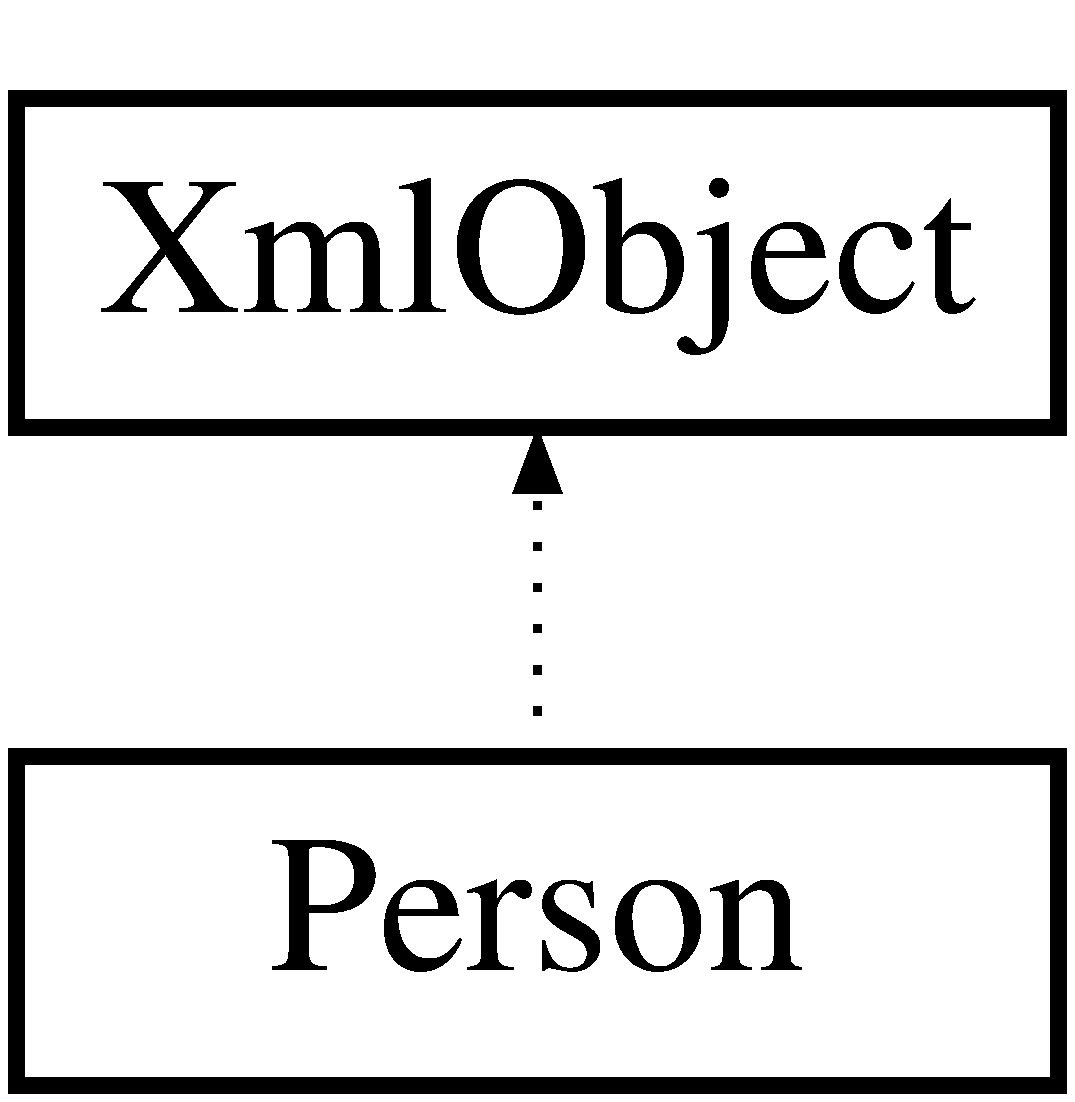
\includegraphics[height=2.000000cm]{classPerson}
\end{center}
\end{figure}
\subsection*{Public Member Functions}
\begin{DoxyCompactItemize}
\item 
\hyperlink{classPerson_a709471c96e7285da132e771e5b319149}{Person} (string, string, char=0, int=0, int=0, string=\char`\"{}friends\char`\"{}, string=\char`\"{}friend\char`\"{}, int=1)
\item 
string \hyperlink{classPerson_a1765bb0876c1fcf995641b35a8b65f54}{to\-\_\-xml} ()
\item 
void \hyperlink{classPerson_aea7c2872014913c743b863a11927cb79}{from\-\_\-xml} (ifstream \&)
\item 
void \hyperlink{classPerson_ad3cdf9ec902f7b024d16534934ce4be0}{wypisz} ()
\item 
string \hyperlink{classPerson_a9826c568c7042e276014b5265a696295}{ret\-\_\-elem} ()
\item 
void \hyperlink{classPerson_a69f7f76d5a500cc45292f25f4ccc9de7}{add\-\_\-pers} (\hyperlink{classXmlObject__string}{Xml\-Object\-\_\-string})
\end{DoxyCompactItemize}
\subsection*{Friends}
\begin{DoxyCompactItemize}
\item 
ifstream \& \hyperlink{classPerson_ac0b416688c8a0b4d3088639af70e83f9}{operator$>$$>$} (ifstream \&, \hyperlink{classPerson}{Person} \&)
\item 
ofstream \& \hyperlink{classPerson_af1cfee572bae052b68a2828ae6a8afb1}{operator$<$$<$} (ofstream \&, \hyperlink{classPerson}{Person})
\item 
ostream \& \hyperlink{classPerson_aba72915725aa68efe29811edaa685801}{operator$<$$<$} (ostream \&, \hyperlink{classPerson}{Person})
\end{DoxyCompactItemize}


\subsection{Detailed Description}
Klasa \hyperlink{classPerson}{Person} dziedziczy po \hyperlink{classXmlObject}{Xml\-Object}. Docelowa struktura sparsowania do formatu X\-M\-L. Posiada wszyskie funkcja do parsowania w formacie X\-M\-L. Zawiera takie informacje jak\-:imie, nazwisko, plec, nr pesel, wzrost, lista znajomych. 

\subsection{Constructor \& Destructor Documentation}
\hypertarget{classPerson_a709471c96e7285da132e771e5b319149}{\index{Person@{Person}!Person@{Person}}
\index{Person@{Person}!Person@{Person}}
\subsubsection[{Person}]{\setlength{\rightskip}{0pt plus 5cm}Person\-::\-Person (
\begin{DoxyParamCaption}
\item[{string}]{xname, }
\item[{string}]{xsurnm, }
\item[{char}]{xsex = {\ttfamily 0}, }
\item[{int}]{x\-Id = {\ttfamily 0}, }
\item[{int}]{xwzrost = {\ttfamily 0}, }
\item[{string}]{xfriends = {\ttfamily \char`\"{}friends\char`\"{}}, }
\item[{string}]{vect\-Elem = {\ttfamily \char`\"{}friend\char`\"{}}, }
\item[{int}]{size = {\ttfamily 1}}
\end{DoxyParamCaption}
)}}\label{classPerson_a709471c96e7285da132e771e5b319149}
Konstruktor. Pozwala ustawic wszystkie atrybuty osoby wedlug koljenosci ich wystepowania. 

\subsection{Member Function Documentation}
\hypertarget{classPerson_a69f7f76d5a500cc45292f25f4ccc9de7}{\index{Person@{Person}!add\-\_\-pers@{add\-\_\-pers}}
\index{add\-\_\-pers@{add\-\_\-pers}!Person@{Person}}
\subsubsection[{add\-\_\-pers}]{\setlength{\rightskip}{0pt plus 5cm}void Person\-::add\-\_\-pers (
\begin{DoxyParamCaption}
\item[{{\bf Xml\-Object\-\_\-string}}]{no}
\end{DoxyParamCaption}
)}}\label{classPerson_a69f7f76d5a500cc45292f25f4ccc9de7}
Funkcja add person. Pozwala dodac nowego przyjaciela do listy. \hypertarget{classPerson_aea7c2872014913c743b863a11927cb79}{\index{Person@{Person}!from\-\_\-xml@{from\-\_\-xml}}
\index{from\-\_\-xml@{from\-\_\-xml}!Person@{Person}}
\subsubsection[{from\-\_\-xml}]{\setlength{\rightskip}{0pt plus 5cm}void Person\-::from\-\_\-xml (
\begin{DoxyParamCaption}
\item[{ifstream \&}]{File}
\end{DoxyParamCaption}
)\hspace{0.3cm}{\ttfamily [virtual]}}}\label{classPerson_aea7c2872014913c743b863a11927cb79}
Funkcja from xml. Wczytuje do obiektu z fomatu X\-M\-L. Argumentem jest zmienna plikowa wskazujaca na O\-T\-W\-A\-R\-T\-Y plik. 

Implements \hyperlink{classXmlObject_a1f45234b87c92b116b5d036875d46d65}{Xml\-Object}.

\hypertarget{classPerson_a9826c568c7042e276014b5265a696295}{\index{Person@{Person}!ret\-\_\-elem@{ret\-\_\-elem}}
\index{ret\-\_\-elem@{ret\-\_\-elem}!Person@{Person}}
\subsubsection[{ret\-\_\-elem}]{\setlength{\rightskip}{0pt plus 5cm}string Person\-::ret\-\_\-elem (
\begin{DoxyParamCaption}
{}
\end{DoxyParamCaption}
)\hspace{0.3cm}{\ttfamily [virtual]}}}\label{classPerson_a9826c568c7042e276014b5265a696295}
Funkcja return element. Zwraca wartosc element. 

Implements \hyperlink{classXmlObject_ae6aa20b1e0ef049e6cc8ddedc2cd8761}{Xml\-Object}.

\hypertarget{classPerson_a1765bb0876c1fcf995641b35a8b65f54}{\index{Person@{Person}!to\-\_\-xml@{to\-\_\-xml}}
\index{to\-\_\-xml@{to\-\_\-xml}!Person@{Person}}
\subsubsection[{to\-\_\-xml}]{\setlength{\rightskip}{0pt plus 5cm}string Person\-::to\-\_\-xml (
\begin{DoxyParamCaption}
{}
\end{DoxyParamCaption}
)\hspace{0.3cm}{\ttfamily [virtual]}}}\label{classPerson_a1765bb0876c1fcf995641b35a8b65f54}
Funkcja to xml. Parsuje obiekt do formatu X\-M\-L i zwraca w postaci napisu(string). 

Implements \hyperlink{classXmlObject_a23b560b6ef62e13cbe227824df5365c3}{Xml\-Object}.

\hypertarget{classPerson_ad3cdf9ec902f7b024d16534934ce4be0}{\index{Person@{Person}!wypisz@{wypisz}}
\index{wypisz@{wypisz}!Person@{Person}}
\subsubsection[{wypisz}]{\setlength{\rightskip}{0pt plus 5cm}void Person\-::wypisz (
\begin{DoxyParamCaption}
{}
\end{DoxyParamCaption}
)}}\label{classPerson_ad3cdf9ec902f7b024d16534934ce4be0}
Funkcja wypisz. Wypisuje cala strukture \hyperlink{classPerson}{Person} w formacie X\-M\-L. 

\subsection{Friends And Related Function Documentation}
\hypertarget{classPerson_af1cfee572bae052b68a2828ae6a8afb1}{\index{Person@{Person}!operator$<$$<$@{operator$<$$<$}}
\index{operator$<$$<$@{operator$<$$<$}!Person@{Person}}
\subsubsection[{operator$<$$<$}]{\setlength{\rightskip}{0pt plus 5cm}ofstream\& operator$<$$<$ (
\begin{DoxyParamCaption}
\item[{ofstream \&}]{File, }
\item[{{\bf Person}}]{p}
\end{DoxyParamCaption}
)\hspace{0.3cm}{\ttfamily [friend]}}}\label{classPerson_af1cfee572bae052b68a2828ae6a8afb1}
Zaprzyjazniony operator. Umozliwia parsowanie do zmiennej plikowej (File) z obiektu (obiekt) uzywajac zapisu\-: File$<$$<$obiekt; \hypertarget{classPerson_aba72915725aa68efe29811edaa685801}{\index{Person@{Person}!operator$<$$<$@{operator$<$$<$}}
\index{operator$<$$<$@{operator$<$$<$}!Person@{Person}}
\subsubsection[{operator$<$$<$}]{\setlength{\rightskip}{0pt plus 5cm}ostream\& operator$<$$<$ (
\begin{DoxyParamCaption}
\item[{ostream \&}]{os, }
\item[{{\bf Person}}]{p}
\end{DoxyParamCaption}
)\hspace{0.3cm}{\ttfamily [friend]}}}\label{classPerson_aba72915725aa68efe29811edaa685801}
Zaprzyjazniony operator. Umozliwia parsowanie do strumienia wyjsciowego (cout) z obiektu (obiekt) uzywajac zapisu\-: cout$<$$<$obiekt; \hypertarget{classPerson_ac0b416688c8a0b4d3088639af70e83f9}{\index{Person@{Person}!operator$>$$>$@{operator$>$$>$}}
\index{operator$>$$>$@{operator$>$$>$}!Person@{Person}}
\subsubsection[{operator$>$$>$}]{\setlength{\rightskip}{0pt plus 5cm}ifstream\& operator$>$$>$ (
\begin{DoxyParamCaption}
\item[{ifstream \&}]{File, }
\item[{{\bf Person} \&}]{p}
\end{DoxyParamCaption}
)\hspace{0.3cm}{\ttfamily [friend]}}}\label{classPerson_ac0b416688c8a0b4d3088639af70e83f9}
Zaprzyjazniony operator. Umozliwia odczyt ze zmiennej plikowej (File) do obiektu (obiekt) uzywajac zapisu\-: File$>$$>$obiekt; Plik musi zawierac strukture w formacie X\-M\-L. 

The documentation for this class was generated from the following files\-:\begin{DoxyCompactItemize}
\item 
\hyperlink{Person_8h}{Person.\-h}\item 
Person.\-cpp\end{DoxyCompactItemize}

\hypertarget{classXmlObject}{\section{Xml\-Object Class Reference}
\label{classXmlObject}\index{Xml\-Object@{Xml\-Object}}
}


{\ttfamily \#include $<$Xml\-Object.\-h$>$}

Inheritance diagram for Xml\-Object\-:\begin{figure}[H]
\begin{center}
\leavevmode
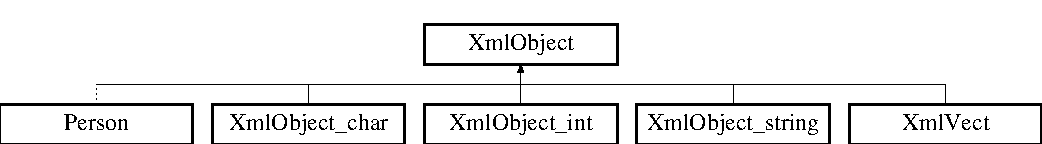
\includegraphics[height=1.931034cm]{classXmlObject}
\end{center}
\end{figure}
\subsection*{Public Member Functions}
\begin{DoxyCompactItemize}
\item 
\hyperlink{classXmlObject_a98b14e9c386ae0aa45a3a99d922c642f}{Xml\-Object} (string)
\item 
virtual \hyperlink{classXmlObject_aa25f0aab0b3f4b9f94185285d6297f20}{$\sim$\-Xml\-Object} ()
\item 
virtual string \hyperlink{classXmlObject_a23b560b6ef62e13cbe227824df5365c3}{to\-\_\-xml} ()=0
\item 
virtual void \hyperlink{classXmlObject_a1f45234b87c92b116b5d036875d46d65}{from\-\_\-xml} (ifstream \&)=0
\item 
virtual string \hyperlink{classXmlObject_ae6aa20b1e0ef049e6cc8ddedc2cd8761}{ret\-\_\-elem} ()=0
\end{DoxyCompactItemize}
\subsection*{Protected Member Functions}
\begin{DoxyCompactItemize}
\item 
void \hyperlink{classXmlObject_a55616473c9f22c01fd3f3d5a31a2a72f}{set\-\_\-elem} (string)
\end{DoxyCompactItemize}
\subsection*{Protected Attributes}
\begin{DoxyCompactItemize}
\item 
string \hyperlink{classXmlObject_a61cc11441cc570e229cd4cf2e8b1736f}{element}
\end{DoxyCompactItemize}


\subsection{Detailed Description}
Klasa \hyperlink{classXmlObject}{Xml\-Object} jest interfejsem. 

\subsection{Constructor \& Destructor Documentation}
\hypertarget{classXmlObject_a98b14e9c386ae0aa45a3a99d922c642f}{\index{Xml\-Object@{Xml\-Object}!Xml\-Object@{Xml\-Object}}
\index{Xml\-Object@{Xml\-Object}!XmlObject@{Xml\-Object}}
\subsubsection[{Xml\-Object}]{\setlength{\rightskip}{0pt plus 5cm}Xml\-Object\-::\-Xml\-Object (
\begin{DoxyParamCaption}
\item[{string}]{xelem}
\end{DoxyParamCaption}
)}}\label{classXmlObject_a98b14e9c386ae0aa45a3a99d922c642f}
Kostruktor. \hypertarget{classXmlObject_aa25f0aab0b3f4b9f94185285d6297f20}{\index{Xml\-Object@{Xml\-Object}!$\sim$\-Xml\-Object@{$\sim$\-Xml\-Object}}
\index{$\sim$\-Xml\-Object@{$\sim$\-Xml\-Object}!XmlObject@{Xml\-Object}}
\subsubsection[{$\sim$\-Xml\-Object}]{\setlength{\rightskip}{0pt plus 5cm}Xml\-Object\-::$\sim$\-Xml\-Object (
\begin{DoxyParamCaption}
{}
\end{DoxyParamCaption}
)\hspace{0.3cm}{\ttfamily [virtual]}}}\label{classXmlObject_aa25f0aab0b3f4b9f94185285d6297f20}
Wirtualny destruktor. 

\subsection{Member Function Documentation}
\hypertarget{classXmlObject_a1f45234b87c92b116b5d036875d46d65}{\index{Xml\-Object@{Xml\-Object}!from\-\_\-xml@{from\-\_\-xml}}
\index{from\-\_\-xml@{from\-\_\-xml}!XmlObject@{Xml\-Object}}
\subsubsection[{from\-\_\-xml}]{\setlength{\rightskip}{0pt plus 5cm}virtual void Xml\-Object\-::from\-\_\-xml (
\begin{DoxyParamCaption}
\item[{ifstream \&}]{}
\end{DoxyParamCaption}
)\hspace{0.3cm}{\ttfamily [pure virtual]}}}\label{classXmlObject_a1f45234b87c92b116b5d036875d46d65}
Funkcja from xml. Sluzy do odczytu struktury z formatu X\-M\-L. Jako argument przyjmuje zmienna plikowa 

Implemented in \hyperlink{classXmlVect_a105c1cd2e05c3f8512d71adbd08e91ac}{Xml\-Vect}, \hyperlink{classXmlObject__char_a06b20ae9d07bd741de017a08895d0da8}{Xml\-Object\-\_\-char}, \hyperlink{classXmlObject__int_a1638d6bef2ad920f60a633f8fd580ab0}{Xml\-Object\-\_\-int}, \hyperlink{classXmlObject__string_a45076d31e063208d1386741f2e1074d3}{Xml\-Object\-\_\-string}, and \hyperlink{classPerson_aea7c2872014913c743b863a11927cb79}{Person}.

\hypertarget{classXmlObject_ae6aa20b1e0ef049e6cc8ddedc2cd8761}{\index{Xml\-Object@{Xml\-Object}!ret\-\_\-elem@{ret\-\_\-elem}}
\index{ret\-\_\-elem@{ret\-\_\-elem}!XmlObject@{Xml\-Object}}
\subsubsection[{ret\-\_\-elem}]{\setlength{\rightskip}{0pt plus 5cm}virtual string Xml\-Object\-::ret\-\_\-elem (
\begin{DoxyParamCaption}
{}
\end{DoxyParamCaption}
)\hspace{0.3cm}{\ttfamily [pure virtual]}}}\label{classXmlObject_ae6aa20b1e0ef049e6cc8ddedc2cd8761}
Funkcja retrun element. Zwraca wartosc zmienna element. 

Implemented in \hyperlink{classXmlVect_a6679bc57a3e6712b99b806f1887e2dc9}{Xml\-Vect}, \hyperlink{classXmlObject__char_a45df01ffd190f0e33f673f2082b0ff8a}{Xml\-Object\-\_\-char}, \hyperlink{classXmlObject__int_a4775d210333968667b9a533fcf2ab1df}{Xml\-Object\-\_\-int}, \hyperlink{classXmlObject__string_a14cc967eb78c9293c49055d54d602717}{Xml\-Object\-\_\-string}, and \hyperlink{classPerson_a9826c568c7042e276014b5265a696295}{Person}.

\hypertarget{classXmlObject_a55616473c9f22c01fd3f3d5a31a2a72f}{\index{Xml\-Object@{Xml\-Object}!set\-\_\-elem@{set\-\_\-elem}}
\index{set\-\_\-elem@{set\-\_\-elem}!XmlObject@{Xml\-Object}}
\subsubsection[{set\-\_\-elem}]{\setlength{\rightskip}{0pt plus 5cm}void Xml\-Object\-::set\-\_\-elem (
\begin{DoxyParamCaption}
\item[{string}]{xelem}
\end{DoxyParamCaption}
)\hspace{0.3cm}{\ttfamily [protected]}}}\label{classXmlObject_a55616473c9f22c01fd3f3d5a31a2a72f}
Funckja set element. Pozwala ustawić nowa wartosc zmiennej element. \hypertarget{classXmlObject_a23b560b6ef62e13cbe227824df5365c3}{\index{Xml\-Object@{Xml\-Object}!to\-\_\-xml@{to\-\_\-xml}}
\index{to\-\_\-xml@{to\-\_\-xml}!XmlObject@{Xml\-Object}}
\subsubsection[{to\-\_\-xml}]{\setlength{\rightskip}{0pt plus 5cm}virtual string Xml\-Object\-::to\-\_\-xml (
\begin{DoxyParamCaption}
{}
\end{DoxyParamCaption}
)\hspace{0.3cm}{\ttfamily [pure virtual]}}}\label{classXmlObject_a23b560b6ef62e13cbe227824df5365c3}
Funkcja to xml. Sluzy do parsowania obiektu do formatu X\-M\-L 

Implemented in \hyperlink{classXmlVect_a5e67ef9b8b9faf9062b6cac413f196a4}{Xml\-Vect}, \hyperlink{classXmlObject__char_a7caa4d2b62ce3240cb6721ca9ac1150d}{Xml\-Object\-\_\-char}, \hyperlink{classXmlObject__int_a071bc574f78dfbb6824cc5a1c5a1e4d7}{Xml\-Object\-\_\-int}, \hyperlink{classXmlObject__string_aea62ae01f9fbbe6718c7269d9dc0591f}{Xml\-Object\-\_\-string}, and \hyperlink{classPerson_a1765bb0876c1fcf995641b35a8b65f54}{Person}.



\subsection{Member Data Documentation}
\hypertarget{classXmlObject_a61cc11441cc570e229cd4cf2e8b1736f}{\index{Xml\-Object@{Xml\-Object}!element@{element}}
\index{element@{element}!XmlObject@{Xml\-Object}}
\subsubsection[{element}]{\setlength{\rightskip}{0pt plus 5cm}string Xml\-Object\-::element\hspace{0.3cm}{\ttfamily [protected]}}}\label{classXmlObject_a61cc11441cc570e229cd4cf2e8b1736f}
element zawiera informacje i nazwie uzywanej struktury. 

The documentation for this class was generated from the following files\-:\begin{DoxyCompactItemize}
\item 
\hyperlink{XmlObject_8h}{Xml\-Object.\-h}\item 
Xml\-Object.\-cpp\end{DoxyCompactItemize}

\hypertarget{classXmlObject__char}{\section{Xml\-Object\-\_\-char Class Reference}
\label{classXmlObject__char}\index{Xml\-Object\-\_\-char@{Xml\-Object\-\_\-char}}
}


{\ttfamily \#include $<$Xml\-Object.\-h$>$}

Inheritance diagram for Xml\-Object\-\_\-char\-:\begin{figure}[H]
\begin{center}
\leavevmode
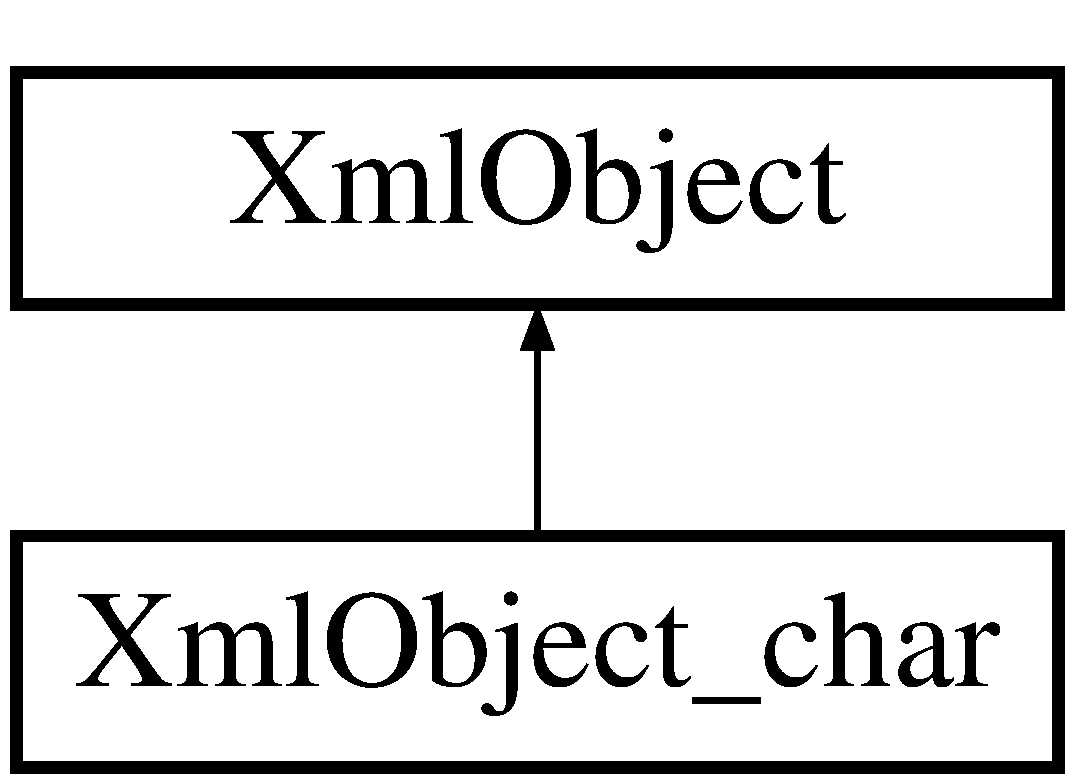
\includegraphics[height=2.000000cm]{classXmlObject__char}
\end{center}
\end{figure}
\subsection*{Public Member Functions}
\begin{DoxyCompactItemize}
\item 
\hyperlink{classXmlObject__char_a593b9a08b971c8b219ffc3a65d224d8d}{Xml\-Object\-\_\-char} (string, char=0)
\item 
virtual string \hyperlink{classXmlObject__char_a7caa4d2b62ce3240cb6721ca9ac1150d}{to\-\_\-xml} ()
\item 
void \hyperlink{classXmlObject__char_a06b20ae9d07bd741de017a08895d0da8}{from\-\_\-xml} (ifstream \&)
\item 
string \hyperlink{classXmlObject__char_a45df01ffd190f0e33f673f2082b0ff8a}{ret\-\_\-elem} ()
\end{DoxyCompactItemize}
\subsection*{Friends}
\begin{DoxyCompactItemize}
\item 
ifstream \& \hyperlink{classXmlObject__char_a5559be49bfe5a30e2e39e19aacf4016d}{operator$>$$>$} (ifstream \&File, \hyperlink{classXmlObject__char}{Xml\-Object\-\_\-char} \&x)
\item 
ofstream \& \hyperlink{classXmlObject__char_a573187365149e426097b27ebbf8e9da3}{operator$<$$<$} (ofstream \&File, \hyperlink{classXmlObject__char}{Xml\-Object\-\_\-char} x)
\item 
ostream \& \hyperlink{classXmlObject__char_a47a42d8624b5b6ce6252d2cf6a815b8a}{operator$<$$<$} (ostream \&os, \hyperlink{classXmlObject__string}{Xml\-Object\-\_\-string} x)
\end{DoxyCompactItemize}
\subsection*{Additional Inherited Members}


\subsection{Detailed Description}
Klasa \hyperlink{classXmlObject__char}{Xml\-Object\-\_\-char} dziedziczy po \hyperlink{classXmlObject}{Xml\-Object}. Przechowuje znaki. Posiada wszytkie metody potrzebne do parsowania do X\-M\-L i odczytu. 

\subsection{Constructor \& Destructor Documentation}
\hypertarget{classXmlObject__char_a593b9a08b971c8b219ffc3a65d224d8d}{\index{Xml\-Object\-\_\-char@{Xml\-Object\-\_\-char}!Xml\-Object\-\_\-char@{Xml\-Object\-\_\-char}}
\index{Xml\-Object\-\_\-char@{Xml\-Object\-\_\-char}!XmlObject_char@{Xml\-Object\-\_\-char}}
\subsubsection[{Xml\-Object\-\_\-char}]{\setlength{\rightskip}{0pt plus 5cm}Xml\-Object\-\_\-char\-::\-Xml\-Object\-\_\-char (
\begin{DoxyParamCaption}
\item[{string}]{xelem, }
\item[{char}]{xmark = {\ttfamily 0}}
\end{DoxyParamCaption}
)}}\label{classXmlObject__char_a593b9a08b971c8b219ffc3a65d224d8d}
Konstruktor. Argumenty\-: wartosc docelowa element, wartosc docelowa mark. Mark domyslnie ustawiane na 0. 

\subsection{Member Function Documentation}
\hypertarget{classXmlObject__char_a06b20ae9d07bd741de017a08895d0da8}{\index{Xml\-Object\-\_\-char@{Xml\-Object\-\_\-char}!from\-\_\-xml@{from\-\_\-xml}}
\index{from\-\_\-xml@{from\-\_\-xml}!XmlObject_char@{Xml\-Object\-\_\-char}}
\subsubsection[{from\-\_\-xml}]{\setlength{\rightskip}{0pt plus 5cm}void Xml\-Object\-\_\-char\-::from\-\_\-xml (
\begin{DoxyParamCaption}
\item[{ifstream \&}]{File}
\end{DoxyParamCaption}
)\hspace{0.3cm}{\ttfamily [virtual]}}}\label{classXmlObject__char_a06b20ae9d07bd741de017a08895d0da8}
Funkcja from xml. Wczytuje do obiektu z fomatu X\-M\-L. Argumentem jest zmienna plikowa wskazujaca na O\-T\-W\-A\-R\-T\-Y plik. 

Implements \hyperlink{classXmlObject_a1f45234b87c92b116b5d036875d46d65}{Xml\-Object}.

\hypertarget{classXmlObject__char_a45df01ffd190f0e33f673f2082b0ff8a}{\index{Xml\-Object\-\_\-char@{Xml\-Object\-\_\-char}!ret\-\_\-elem@{ret\-\_\-elem}}
\index{ret\-\_\-elem@{ret\-\_\-elem}!XmlObject_char@{Xml\-Object\-\_\-char}}
\subsubsection[{ret\-\_\-elem}]{\setlength{\rightskip}{0pt plus 5cm}string Xml\-Object\-\_\-char\-::ret\-\_\-elem (
\begin{DoxyParamCaption}
{}
\end{DoxyParamCaption}
)\hspace{0.3cm}{\ttfamily [virtual]}}}\label{classXmlObject__char_a45df01ffd190f0e33f673f2082b0ff8a}
Funkcja return element. Zwraca wartosc element. 

Implements \hyperlink{classXmlObject_ae6aa20b1e0ef049e6cc8ddedc2cd8761}{Xml\-Object}.

\hypertarget{classXmlObject__char_a7caa4d2b62ce3240cb6721ca9ac1150d}{\index{Xml\-Object\-\_\-char@{Xml\-Object\-\_\-char}!to\-\_\-xml@{to\-\_\-xml}}
\index{to\-\_\-xml@{to\-\_\-xml}!XmlObject_char@{Xml\-Object\-\_\-char}}
\subsubsection[{to\-\_\-xml}]{\setlength{\rightskip}{0pt plus 5cm}string Xml\-Object\-\_\-char\-::to\-\_\-xml (
\begin{DoxyParamCaption}
{}
\end{DoxyParamCaption}
)\hspace{0.3cm}{\ttfamily [virtual]}}}\label{classXmlObject__char_a7caa4d2b62ce3240cb6721ca9ac1150d}
Funkcja to xml. Parsuje obiekt do formatu X\-M\-L i zwraca w postaci napisu(string). 

Implements \hyperlink{classXmlObject_a23b560b6ef62e13cbe227824df5365c3}{Xml\-Object}.



\subsection{Friends And Related Function Documentation}
\hypertarget{classXmlObject__char_a573187365149e426097b27ebbf8e9da3}{\index{Xml\-Object\-\_\-char@{Xml\-Object\-\_\-char}!operator$<$$<$@{operator$<$$<$}}
\index{operator$<$$<$@{operator$<$$<$}!XmlObject_char@{Xml\-Object\-\_\-char}}
\subsubsection[{operator$<$$<$}]{\setlength{\rightskip}{0pt plus 5cm}ofstream\& operator$<$$<$ (
\begin{DoxyParamCaption}
\item[{ofstream \&}]{File, }
\item[{{\bf Xml\-Object\-\_\-char}}]{x}
\end{DoxyParamCaption}
)\hspace{0.3cm}{\ttfamily [friend]}}}\label{classXmlObject__char_a573187365149e426097b27ebbf8e9da3}
Zaprzyjazniony operator. Umozliwia parsowanie do zmiennej plikowej (File) z obiektu (obiekt) uzywajac zapisu\-: File$<$$<$obiekt; \hypertarget{classXmlObject__char_a47a42d8624b5b6ce6252d2cf6a815b8a}{\index{Xml\-Object\-\_\-char@{Xml\-Object\-\_\-char}!operator$<$$<$@{operator$<$$<$}}
\index{operator$<$$<$@{operator$<$$<$}!XmlObject_char@{Xml\-Object\-\_\-char}}
\subsubsection[{operator$<$$<$}]{\setlength{\rightskip}{0pt plus 5cm}ostream\& operator$<$$<$ (
\begin{DoxyParamCaption}
\item[{ostream \&}]{os, }
\item[{{\bf Xml\-Object\-\_\-string}}]{x}
\end{DoxyParamCaption}
)\hspace{0.3cm}{\ttfamily [friend]}}}\label{classXmlObject__char_a47a42d8624b5b6ce6252d2cf6a815b8a}
Zaprzyjazniony operator. Umozliwia parsowanie do strumienia wyjsciowego (cout) z obiektu (obiekt) uzywajac zapisu\-: cout$<$$<$obiekt; \hypertarget{classXmlObject__char_a5559be49bfe5a30e2e39e19aacf4016d}{\index{Xml\-Object\-\_\-char@{Xml\-Object\-\_\-char}!operator$>$$>$@{operator$>$$>$}}
\index{operator$>$$>$@{operator$>$$>$}!XmlObject_char@{Xml\-Object\-\_\-char}}
\subsubsection[{operator$>$$>$}]{\setlength{\rightskip}{0pt plus 5cm}ifstream\& operator$>$$>$ (
\begin{DoxyParamCaption}
\item[{ifstream \&}]{File, }
\item[{{\bf Xml\-Object\-\_\-char} \&}]{x}
\end{DoxyParamCaption}
)\hspace{0.3cm}{\ttfamily [friend]}}}\label{classXmlObject__char_a5559be49bfe5a30e2e39e19aacf4016d}
Zaprzyjazniony operator. Umozliwia odczyt ze zmiennej plikowej (File) do obiektu (obiekt) uzywajac zapisu\-: File$>$$>$obiekt; Plik musi zawierac strukture w formacie X\-M\-L. 

The documentation for this class was generated from the following files\-:\begin{DoxyCompactItemize}
\item 
\hyperlink{XmlObject_8h}{Xml\-Object.\-h}\item 
Xml\-Object.\-cpp\end{DoxyCompactItemize}

\hypertarget{classXmlObject__int}{\section{Xml\-Object\-\_\-int Class Reference}
\label{classXmlObject__int}\index{Xml\-Object\-\_\-int@{Xml\-Object\-\_\-int}}
}


{\ttfamily \#include $<$Xml\-Object.\-h$>$}

Inheritance diagram for Xml\-Object\-\_\-int\-:\begin{figure}[H]
\begin{center}
\leavevmode
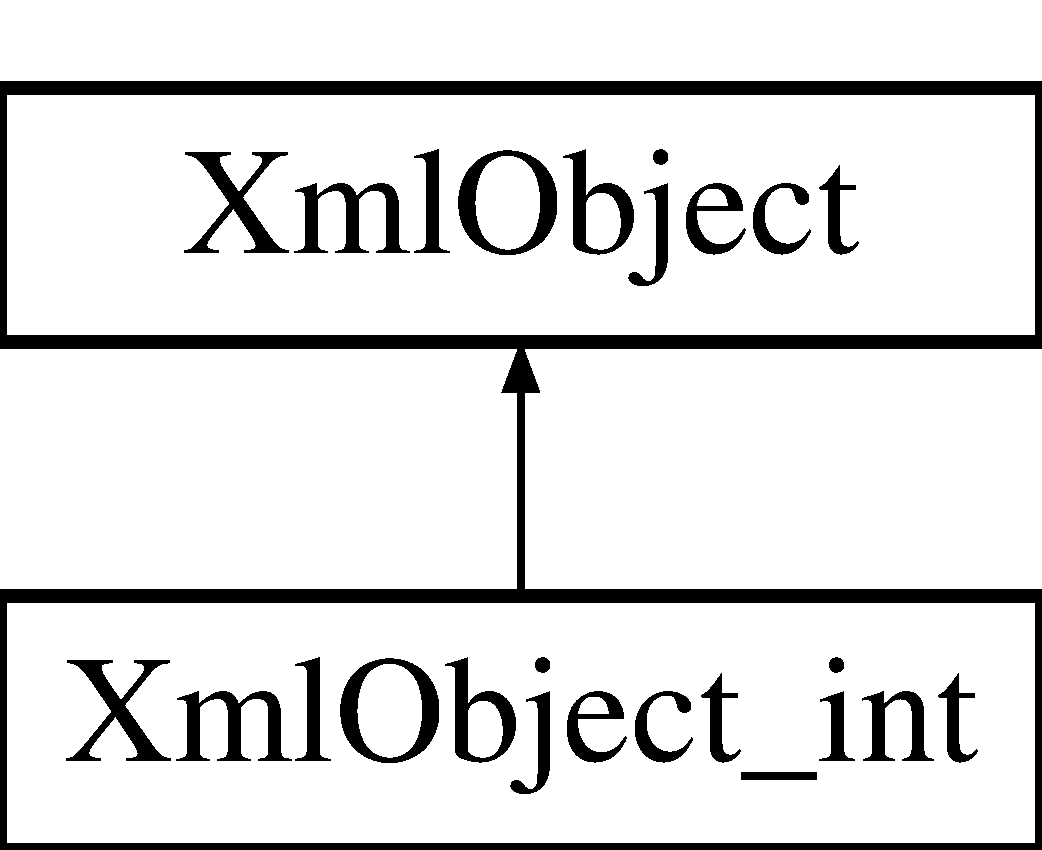
\includegraphics[height=2.000000cm]{classXmlObject__int}
\end{center}
\end{figure}
\subsection*{Public Member Functions}
\begin{DoxyCompactItemize}
\item 
\hyperlink{classXmlObject__int_a20c9fc3a3785e8c4c07f7b2ac86a4cbd}{Xml\-Object\-\_\-int} (string, int=0)
\item 
virtual string \hyperlink{classXmlObject__int_a071bc574f78dfbb6824cc5a1c5a1e4d7}{to\-\_\-xml} ()
\item 
void \hyperlink{classXmlObject__int_a1638d6bef2ad920f60a633f8fd580ab0}{from\-\_\-xml} (ifstream \&)
\item 
string \hyperlink{classXmlObject__int_a4775d210333968667b9a533fcf2ab1df}{ret\-\_\-elem} ()
\item 
int \hyperlink{classXmlObject__int_a2c5b3031f04cc9ed0b343ab057aa0022}{ret\-\_\-value} ()
\item 
void \hyperlink{classXmlObject__int_a70573ff274498cd00ce2ed54e4391f7f}{set\-\_\-value} (int)
\end{DoxyCompactItemize}
\subsection*{Friends}
\begin{DoxyCompactItemize}
\item 
ifstream \& \hyperlink{classXmlObject__int_af6602349819f033b38c8214cbdaf1806}{operator$>$$>$} (ifstream \&File, \hyperlink{classXmlObject__int}{Xml\-Object\-\_\-int} \&x)
\item 
ofstream \& \hyperlink{classXmlObject__int_a6c347c380c359066d322373333dc88b7}{operator$<$$<$} (ofstream \&File, \hyperlink{classXmlObject__int}{Xml\-Object\-\_\-int} x)
\item 
ostream \& \hyperlink{classXmlObject__int_a47a42d8624b5b6ce6252d2cf6a815b8a}{operator$<$$<$} (ostream \&os, \hyperlink{classXmlObject__string}{Xml\-Object\-\_\-string} x)
\end{DoxyCompactItemize}
\subsection*{Additional Inherited Members}


\subsection{Detailed Description}
Klasa \hyperlink{classXmlObject__int}{Xml\-Object\-\_\-int} dziedziczy po \hyperlink{classXmlObject}{Xml\-Object}. Przechowuje liczby calkowite. Posiada wszytkie metody potrzebne do parsowania do X\-M\-L i odczytu. 

\subsection{Constructor \& Destructor Documentation}
\hypertarget{classXmlObject__int_a20c9fc3a3785e8c4c07f7b2ac86a4cbd}{\index{Xml\-Object\-\_\-int@{Xml\-Object\-\_\-int}!Xml\-Object\-\_\-int@{Xml\-Object\-\_\-int}}
\index{Xml\-Object\-\_\-int@{Xml\-Object\-\_\-int}!XmlObject_int@{Xml\-Object\-\_\-int}}
\subsubsection[{Xml\-Object\-\_\-int}]{\setlength{\rightskip}{0pt plus 5cm}Xml\-Object\-\_\-int\-::\-Xml\-Object\-\_\-int (
\begin{DoxyParamCaption}
\item[{string}]{xelem, }
\item[{int}]{x = {\ttfamily 0}}
\end{DoxyParamCaption}
)}}\label{classXmlObject__int_a20c9fc3a3785e8c4c07f7b2ac86a4cbd}
Konstruktor. Argumenty\-: wartosc docelowa element, wartosc docelowa value. Value domyslnie ustawiane na 0. 

\subsection{Member Function Documentation}
\hypertarget{classXmlObject__int_a1638d6bef2ad920f60a633f8fd580ab0}{\index{Xml\-Object\-\_\-int@{Xml\-Object\-\_\-int}!from\-\_\-xml@{from\-\_\-xml}}
\index{from\-\_\-xml@{from\-\_\-xml}!XmlObject_int@{Xml\-Object\-\_\-int}}
\subsubsection[{from\-\_\-xml}]{\setlength{\rightskip}{0pt plus 5cm}void Xml\-Object\-\_\-int\-::from\-\_\-xml (
\begin{DoxyParamCaption}
\item[{ifstream \&}]{File}
\end{DoxyParamCaption}
)\hspace{0.3cm}{\ttfamily [virtual]}}}\label{classXmlObject__int_a1638d6bef2ad920f60a633f8fd580ab0}
Funkcja from xml. Wczytuje do obiektu z fomatu X\-M\-L. Argumentem jest zmienna plikowa wskazujaca na O\-T\-W\-A\-R\-T\-Y plik. 

Implements \hyperlink{classXmlObject_a1f45234b87c92b116b5d036875d46d65}{Xml\-Object}.

\hypertarget{classXmlObject__int_a4775d210333968667b9a533fcf2ab1df}{\index{Xml\-Object\-\_\-int@{Xml\-Object\-\_\-int}!ret\-\_\-elem@{ret\-\_\-elem}}
\index{ret\-\_\-elem@{ret\-\_\-elem}!XmlObject_int@{Xml\-Object\-\_\-int}}
\subsubsection[{ret\-\_\-elem}]{\setlength{\rightskip}{0pt plus 5cm}string Xml\-Object\-\_\-int\-::ret\-\_\-elem (
\begin{DoxyParamCaption}
{}
\end{DoxyParamCaption}
)\hspace{0.3cm}{\ttfamily [virtual]}}}\label{classXmlObject__int_a4775d210333968667b9a533fcf2ab1df}
Funkcja return element. Zwraca wartosc element. 

Implements \hyperlink{classXmlObject_ae6aa20b1e0ef049e6cc8ddedc2cd8761}{Xml\-Object}.

\hypertarget{classXmlObject__int_a2c5b3031f04cc9ed0b343ab057aa0022}{\index{Xml\-Object\-\_\-int@{Xml\-Object\-\_\-int}!ret\-\_\-value@{ret\-\_\-value}}
\index{ret\-\_\-value@{ret\-\_\-value}!XmlObject_int@{Xml\-Object\-\_\-int}}
\subsubsection[{ret\-\_\-value}]{\setlength{\rightskip}{0pt plus 5cm}int Xml\-Object\-\_\-int\-::ret\-\_\-value (
\begin{DoxyParamCaption}
{}
\end{DoxyParamCaption}
)}}\label{classXmlObject__int_a2c5b3031f04cc9ed0b343ab057aa0022}
Funkcja return value. Zwraca wartosc zmiennej value. \hypertarget{classXmlObject__int_a70573ff274498cd00ce2ed54e4391f7f}{\index{Xml\-Object\-\_\-int@{Xml\-Object\-\_\-int}!set\-\_\-value@{set\-\_\-value}}
\index{set\-\_\-value@{set\-\_\-value}!XmlObject_int@{Xml\-Object\-\_\-int}}
\subsubsection[{set\-\_\-value}]{\setlength{\rightskip}{0pt plus 5cm}void Xml\-Object\-\_\-int\-::set\-\_\-value (
\begin{DoxyParamCaption}
\item[{int}]{x}
\end{DoxyParamCaption}
)}}\label{classXmlObject__int_a70573ff274498cd00ce2ed54e4391f7f}
Funkcja set value. Ustawia wartosc value na ta podane w argumencie. \hypertarget{classXmlObject__int_a071bc574f78dfbb6824cc5a1c5a1e4d7}{\index{Xml\-Object\-\_\-int@{Xml\-Object\-\_\-int}!to\-\_\-xml@{to\-\_\-xml}}
\index{to\-\_\-xml@{to\-\_\-xml}!XmlObject_int@{Xml\-Object\-\_\-int}}
\subsubsection[{to\-\_\-xml}]{\setlength{\rightskip}{0pt plus 5cm}string Xml\-Object\-\_\-int\-::to\-\_\-xml (
\begin{DoxyParamCaption}
{}
\end{DoxyParamCaption}
)\hspace{0.3cm}{\ttfamily [virtual]}}}\label{classXmlObject__int_a071bc574f78dfbb6824cc5a1c5a1e4d7}
Funkcja to xml. Parsuje obiekt do formatu X\-M\-L i zwraca w postaci napisu(string). 

Implements \hyperlink{classXmlObject_a23b560b6ef62e13cbe227824df5365c3}{Xml\-Object}.



\subsection{Friends And Related Function Documentation}
\hypertarget{classXmlObject__int_a6c347c380c359066d322373333dc88b7}{\index{Xml\-Object\-\_\-int@{Xml\-Object\-\_\-int}!operator$<$$<$@{operator$<$$<$}}
\index{operator$<$$<$@{operator$<$$<$}!XmlObject_int@{Xml\-Object\-\_\-int}}
\subsubsection[{operator$<$$<$}]{\setlength{\rightskip}{0pt plus 5cm}ofstream\& operator$<$$<$ (
\begin{DoxyParamCaption}
\item[{ofstream \&}]{File, }
\item[{{\bf Xml\-Object\-\_\-int}}]{x}
\end{DoxyParamCaption}
)\hspace{0.3cm}{\ttfamily [friend]}}}\label{classXmlObject__int_a6c347c380c359066d322373333dc88b7}
Zaprzyjazniony operator. Umozliwia parsowanie do zmiennej plikowej (File) z obiektu (obiekt) uzywajac zapisu\-: File$<$$<$obiekt; \hypertarget{classXmlObject__int_a47a42d8624b5b6ce6252d2cf6a815b8a}{\index{Xml\-Object\-\_\-int@{Xml\-Object\-\_\-int}!operator$<$$<$@{operator$<$$<$}}
\index{operator$<$$<$@{operator$<$$<$}!XmlObject_int@{Xml\-Object\-\_\-int}}
\subsubsection[{operator$<$$<$}]{\setlength{\rightskip}{0pt plus 5cm}ostream\& operator$<$$<$ (
\begin{DoxyParamCaption}
\item[{ostream \&}]{os, }
\item[{{\bf Xml\-Object\-\_\-string}}]{x}
\end{DoxyParamCaption}
)\hspace{0.3cm}{\ttfamily [friend]}}}\label{classXmlObject__int_a47a42d8624b5b6ce6252d2cf6a815b8a}
Zaprzyjazniony operator. Umozliwia parsowanie do strumienia wyjsciowego (cout) z obiektu (obiekt) uzywajac zapisu\-: cout$<$$<$obiekt; \hypertarget{classXmlObject__int_af6602349819f033b38c8214cbdaf1806}{\index{Xml\-Object\-\_\-int@{Xml\-Object\-\_\-int}!operator$>$$>$@{operator$>$$>$}}
\index{operator$>$$>$@{operator$>$$>$}!XmlObject_int@{Xml\-Object\-\_\-int}}
\subsubsection[{operator$>$$>$}]{\setlength{\rightskip}{0pt plus 5cm}ifstream\& operator$>$$>$ (
\begin{DoxyParamCaption}
\item[{ifstream \&}]{File, }
\item[{{\bf Xml\-Object\-\_\-int} \&}]{x}
\end{DoxyParamCaption}
)\hspace{0.3cm}{\ttfamily [friend]}}}\label{classXmlObject__int_af6602349819f033b38c8214cbdaf1806}
Zaprzyjazniony operator. Umozliwia odczyt ze zmiennej plikowej (File) do obiektu (obiekt) uzywajac zapisu\-: File$>$$>$obiekt; Plik musi zawierac strukture w formacie X\-M\-L. 

The documentation for this class was generated from the following files\-:\begin{DoxyCompactItemize}
\item 
\hyperlink{XmlObject_8h}{Xml\-Object.\-h}\item 
Xml\-Object.\-cpp\end{DoxyCompactItemize}

\hypertarget{classXmlObject__string}{\section{Xml\-Object\-\_\-string Class Reference}
\label{classXmlObject__string}\index{Xml\-Object\-\_\-string@{Xml\-Object\-\_\-string}}
}


{\ttfamily \#include $<$Xml\-Object.\-h$>$}

Inheritance diagram for Xml\-Object\-\_\-string\-:\begin{figure}[H]
\begin{center}
\leavevmode
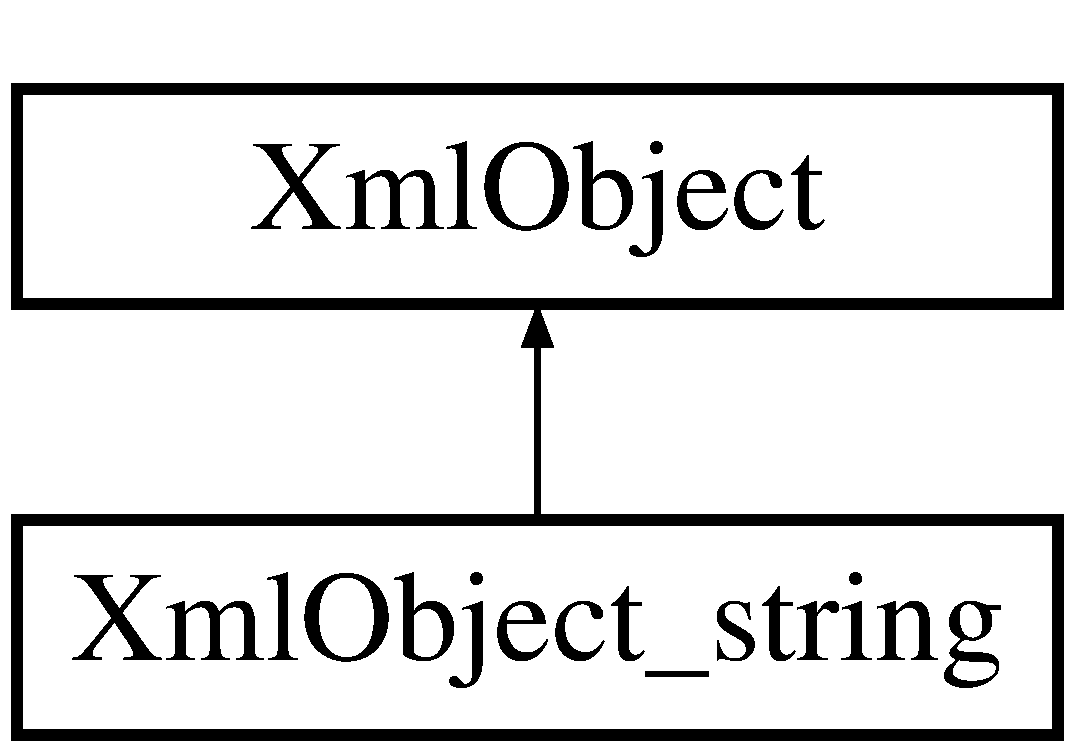
\includegraphics[height=2.000000cm]{classXmlObject__string}
\end{center}
\end{figure}
\subsection*{Public Member Functions}
\begin{DoxyCompactItemize}
\item 
\hyperlink{classXmlObject__string_af8235aac95dee8af1d4ad9f058865948}{Xml\-Object\-\_\-string} (string=\char`\"{}\textbackslash{}0\char`\"{}, string=\char`\"{}\textbackslash{}0\char`\"{})
\item 
string \hyperlink{classXmlObject__string_aea62ae01f9fbbe6718c7269d9dc0591f}{to\-\_\-xml} ()
\item 
void \hyperlink{classXmlObject__string_a45076d31e063208d1386741f2e1074d3}{from\-\_\-xml} (ifstream \&)
\item 
string \hyperlink{classXmlObject__string_a14cc967eb78c9293c49055d54d602717}{ret\-\_\-elem} ()
\item 
void \hyperlink{classXmlObject__string_a41323b0a911aab6145da0ec527329c4a}{set\-\_\-elem} (string)
\end{DoxyCompactItemize}
\subsection*{Friends}
\begin{DoxyCompactItemize}
\item 
ifstream \& \hyperlink{classXmlObject__string_a5790a0bb79553d3597a8498aaf8118a2}{operator$>$$>$} (ifstream \&File, \hyperlink{classXmlObject__string}{Xml\-Object\-\_\-string} \&x)
\item 
ofstream \& \hyperlink{classXmlObject__string_acf1a3de06b876cac2c8b5ae510d13620}{operator$<$$<$} (ofstream \&File, \hyperlink{classXmlObject__string}{Xml\-Object\-\_\-string} x)
\item 
ostream \& \hyperlink{classXmlObject__string_a47a42d8624b5b6ce6252d2cf6a815b8a}{operator$<$$<$} (ostream \&os, \hyperlink{classXmlObject__string}{Xml\-Object\-\_\-string} x)
\end{DoxyCompactItemize}
\subsection*{Additional Inherited Members}


\subsection{Detailed Description}
Klasa \hyperlink{classXmlObject__string}{Xml\-Object\-\_\-string} i dziedziczy po klasie \hyperlink{classXmlObject}{Xml\-Object}. Przechowuje napisy. Zawiera zmienna klasy string i wszystkie metody sluzace parsowaniu jej do formatu X\-M\-L. 

\subsection{Constructor \& Destructor Documentation}
\hypertarget{classXmlObject__string_af8235aac95dee8af1d4ad9f058865948}{\index{Xml\-Object\-\_\-string@{Xml\-Object\-\_\-string}!Xml\-Object\-\_\-string@{Xml\-Object\-\_\-string}}
\index{Xml\-Object\-\_\-string@{Xml\-Object\-\_\-string}!XmlObject_string@{Xml\-Object\-\_\-string}}
\subsubsection[{Xml\-Object\-\_\-string}]{\setlength{\rightskip}{0pt plus 5cm}Xml\-Object\-\_\-string\-::\-Xml\-Object\-\_\-string (
\begin{DoxyParamCaption}
\item[{string}]{xelem = {\ttfamily \char`\"{}\textbackslash{}0\char`\"{}}, }
\item[{string}]{xname = {\ttfamily \char`\"{}\textbackslash{}0\char`\"{}}}
\end{DoxyParamCaption}
)}}\label{classXmlObject__string_af8235aac95dee8af1d4ad9f058865948}
Kostruktor. Jego argumenty zawieraja wartosci zmiennych kolejno\-:element, name. Domyślnie ustawiane sa na wskazniki zerowe. 

\subsection{Member Function Documentation}
\hypertarget{classXmlObject__string_a45076d31e063208d1386741f2e1074d3}{\index{Xml\-Object\-\_\-string@{Xml\-Object\-\_\-string}!from\-\_\-xml@{from\-\_\-xml}}
\index{from\-\_\-xml@{from\-\_\-xml}!XmlObject_string@{Xml\-Object\-\_\-string}}
\subsubsection[{from\-\_\-xml}]{\setlength{\rightskip}{0pt plus 5cm}void Xml\-Object\-\_\-string\-::from\-\_\-xml (
\begin{DoxyParamCaption}
\item[{ifstream \&}]{File}
\end{DoxyParamCaption}
)\hspace{0.3cm}{\ttfamily [virtual]}}}\label{classXmlObject__string_a45076d31e063208d1386741f2e1074d3}
Funkcja from xml. Wczytuje zawartosc struktury z formatu X\-M\-L. Jak argument przyjmuje zmienna plikowa wskazujaca na O\-T\-W\-A\-R\-T\-Y plik. 

Implements \hyperlink{classXmlObject_a1f45234b87c92b116b5d036875d46d65}{Xml\-Object}.

\hypertarget{classXmlObject__string_a14cc967eb78c9293c49055d54d602717}{\index{Xml\-Object\-\_\-string@{Xml\-Object\-\_\-string}!ret\-\_\-elem@{ret\-\_\-elem}}
\index{ret\-\_\-elem@{ret\-\_\-elem}!XmlObject_string@{Xml\-Object\-\_\-string}}
\subsubsection[{ret\-\_\-elem}]{\setlength{\rightskip}{0pt plus 5cm}string Xml\-Object\-\_\-string\-::ret\-\_\-elem (
\begin{DoxyParamCaption}
{}
\end{DoxyParamCaption}
)\hspace{0.3cm}{\ttfamily [virtual]}}}\label{classXmlObject__string_a14cc967eb78c9293c49055d54d602717}
Funkcja return element. Zwraca wartosc zmiennaj element. 

Implements \hyperlink{classXmlObject_ae6aa20b1e0ef049e6cc8ddedc2cd8761}{Xml\-Object}.

\hypertarget{classXmlObject__string_a41323b0a911aab6145da0ec527329c4a}{\index{Xml\-Object\-\_\-string@{Xml\-Object\-\_\-string}!set\-\_\-elem@{set\-\_\-elem}}
\index{set\-\_\-elem@{set\-\_\-elem}!XmlObject_string@{Xml\-Object\-\_\-string}}
\subsubsection[{set\-\_\-elem}]{\setlength{\rightskip}{0pt plus 5cm}void Xml\-Object\-\_\-string\-::set\-\_\-elem (
\begin{DoxyParamCaption}
\item[{string}]{xelem}
\end{DoxyParamCaption}
)}}\label{classXmlObject__string_a41323b0a911aab6145da0ec527329c4a}
Funkcja set element. Ustawia wartosc element na wartosc podana w argumencie. \hypertarget{classXmlObject__string_aea62ae01f9fbbe6718c7269d9dc0591f}{\index{Xml\-Object\-\_\-string@{Xml\-Object\-\_\-string}!to\-\_\-xml@{to\-\_\-xml}}
\index{to\-\_\-xml@{to\-\_\-xml}!XmlObject_string@{Xml\-Object\-\_\-string}}
\subsubsection[{to\-\_\-xml}]{\setlength{\rightskip}{0pt plus 5cm}string Xml\-Object\-\_\-string\-::to\-\_\-xml (
\begin{DoxyParamCaption}
{}
\end{DoxyParamCaption}
)\hspace{0.3cm}{\ttfamily [virtual]}}}\label{classXmlObject__string_aea62ae01f9fbbe6718c7269d9dc0591f}
Funkcja to xml. Nie przyjmuje argumentow. Parsuje obiekt do formatu X\-M\-L ($<$element$>$name$<$/element$>$) 

Implements \hyperlink{classXmlObject_a23b560b6ef62e13cbe227824df5365c3}{Xml\-Object}.



\subsection{Friends And Related Function Documentation}
\hypertarget{classXmlObject__string_acf1a3de06b876cac2c8b5ae510d13620}{\index{Xml\-Object\-\_\-string@{Xml\-Object\-\_\-string}!operator$<$$<$@{operator$<$$<$}}
\index{operator$<$$<$@{operator$<$$<$}!XmlObject_string@{Xml\-Object\-\_\-string}}
\subsubsection[{operator$<$$<$}]{\setlength{\rightskip}{0pt plus 5cm}ofstream\& operator$<$$<$ (
\begin{DoxyParamCaption}
\item[{ofstream \&}]{File, }
\item[{{\bf Xml\-Object\-\_\-string}}]{x}
\end{DoxyParamCaption}
)\hspace{0.3cm}{\ttfamily [friend]}}}\label{classXmlObject__string_acf1a3de06b876cac2c8b5ae510d13620}
Zaprzyjazniony operator. Umozliwia parsowanie do zmiennej plikowej (File) z obiektu (obiekt) uzywajac zapisu\-: File$<$$<$obiekt; Zapisywanie jest do formatu X\-M\-L. \hypertarget{classXmlObject__string_a47a42d8624b5b6ce6252d2cf6a815b8a}{\index{Xml\-Object\-\_\-string@{Xml\-Object\-\_\-string}!operator$<$$<$@{operator$<$$<$}}
\index{operator$<$$<$@{operator$<$$<$}!XmlObject_string@{Xml\-Object\-\_\-string}}
\subsubsection[{operator$<$$<$}]{\setlength{\rightskip}{0pt plus 5cm}ostream\& operator$<$$<$ (
\begin{DoxyParamCaption}
\item[{ostream \&}]{os, }
\item[{{\bf Xml\-Object\-\_\-string}}]{x}
\end{DoxyParamCaption}
)\hspace{0.3cm}{\ttfamily [friend]}}}\label{classXmlObject__string_a47a42d8624b5b6ce6252d2cf6a815b8a}
Zaprzyjazniony operator. Umozliwia parsowanie do strumienia wyjsciowego (cout) z obiektu (obiekt) uzywajac zapisu\-: cout$<$$<$obiekt; \hypertarget{classXmlObject__string_a5790a0bb79553d3597a8498aaf8118a2}{\index{Xml\-Object\-\_\-string@{Xml\-Object\-\_\-string}!operator$>$$>$@{operator$>$$>$}}
\index{operator$>$$>$@{operator$>$$>$}!XmlObject_string@{Xml\-Object\-\_\-string}}
\subsubsection[{operator$>$$>$}]{\setlength{\rightskip}{0pt plus 5cm}ifstream\& operator$>$$>$ (
\begin{DoxyParamCaption}
\item[{ifstream \&}]{File, }
\item[{{\bf Xml\-Object\-\_\-string} \&}]{x}
\end{DoxyParamCaption}
)\hspace{0.3cm}{\ttfamily [friend]}}}\label{classXmlObject__string_a5790a0bb79553d3597a8498aaf8118a2}
Zaprzyjazniony operator. Umozliwia odczyt ze zmiennej plikowej (File) do obiektu (obiekt) uzywajac zapisu\-: File$>$$>$obiekt; Plik musi zawierac strukture w formacie X\-M\-L. 

The documentation for this class was generated from the following files\-:\begin{DoxyCompactItemize}
\item 
\hyperlink{XmlObject_8h}{Xml\-Object.\-h}\item 
Xml\-Object.\-cpp\end{DoxyCompactItemize}

\hypertarget{classXmlVect}{\section{Xml\-Vect Class Reference}
\label{classXmlVect}\index{Xml\-Vect@{Xml\-Vect}}
}


{\ttfamily \#include $<$Xml\-Object.\-h$>$}

Inheritance diagram for Xml\-Vect\-:\begin{figure}[H]
\begin{center}
\leavevmode
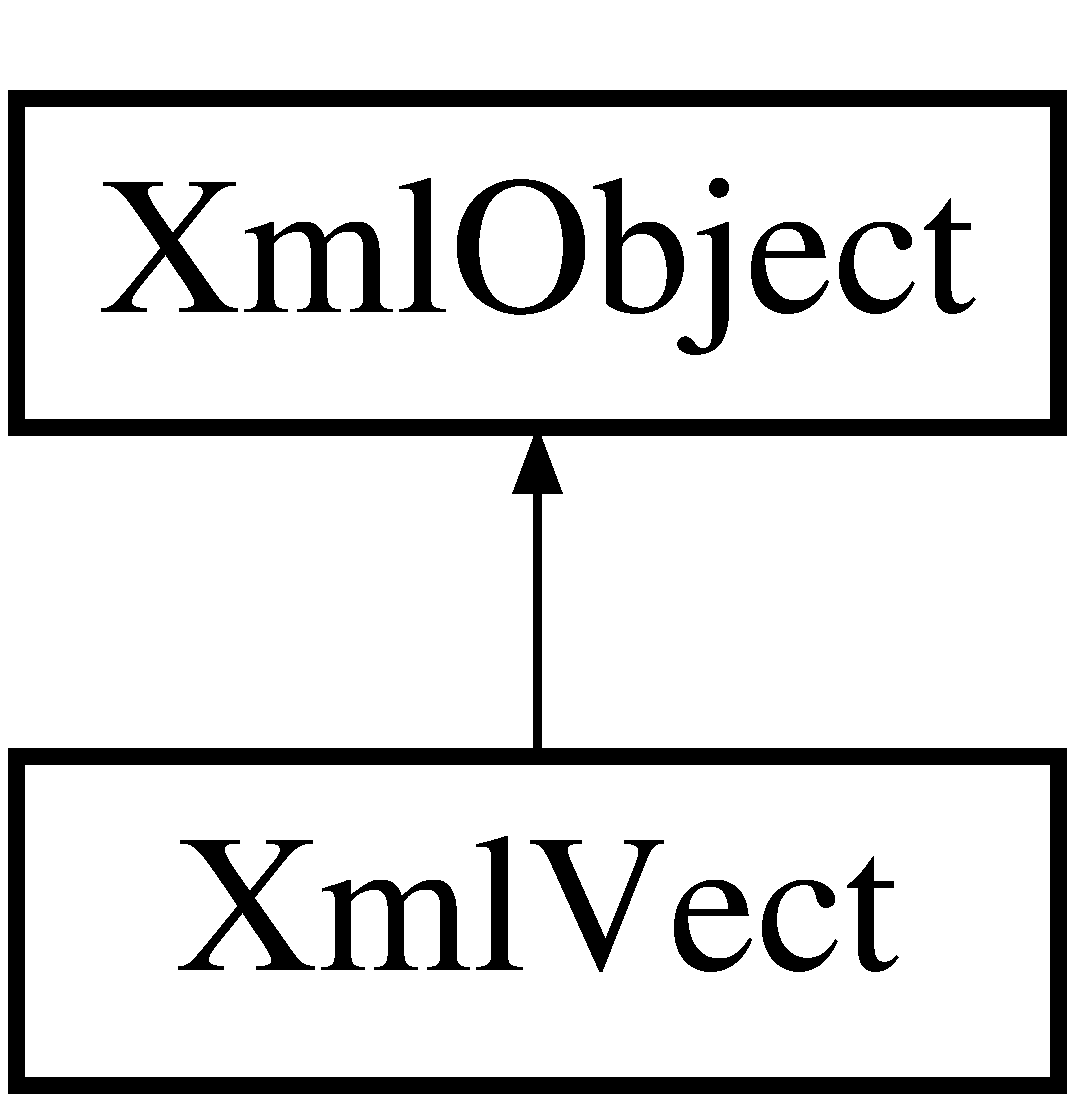
\includegraphics[height=2.000000cm]{classXmlVect}
\end{center}
\end{figure}
\subsection*{Public Member Functions}
\begin{DoxyCompactItemize}
\item 
\hyperlink{classXmlVect_a031b710cdcc779a696040b98f21381e4}{Xml\-Vect} (string, string, int)
\item 
\hyperlink{classXmlVect_a0a27cde8a84f647d128260ac5df76165}{$\sim$\-Xml\-Vect} ()
\item 
\hypertarget{classXmlVect_ac8b30d8d46632736cbcce093231f89bc}{void {\bfseries set\-\_\-elem} (string, string)}\label{classXmlVect_ac8b30d8d46632736cbcce093231f89bc}

\item 
string \hyperlink{classXmlVect_a6679bc57a3e6712b99b806f1887e2dc9}{ret\-\_\-elem} ()
\item 
bool \hyperlink{classXmlVect_aa8c43c842aad1b0aa7722f7eaf2245ef}{push} (\hyperlink{classXmlObject__string}{Xml\-Object\-\_\-string})
\item 
bool \hyperlink{classXmlVect_af89d6523826f072d67f131d0ba4312aa}{remove} ()
\item 
string \hyperlink{classXmlVect_a5e67ef9b8b9faf9062b6cac413f196a4}{to\-\_\-xml} ()
\item 
void \hyperlink{classXmlVect_a105c1cd2e05c3f8512d71adbd08e91ac}{from\-\_\-xml} (ifstream \&)
\end{DoxyCompactItemize}
\subsection*{Additional Inherited Members}


\subsection{Detailed Description}
Klasa \hyperlink{classXmlVect}{Xml\-Vect} dziedzieczy po \hyperlink{classXmlObject}{Xml\-Object}. Zawiera tablice obiektow \hyperlink{classXmlObject__string}{Xml\-Object\-\_\-string}. Posiada wszytkie metody potrzebne do parsowania do X\-M\-L i odczytu. Zapis ma forme\-: $<$element$>$ $<$\-S\-I\-Z\-E$>$...$<$/\-S\-I\-Z\-E$>$ $<$Tab\mbox{[}0\mbox{]}.element$>$Tab\mbox{[}0\mbox{]}.name$<$/\-Tab\mbox{[}0\mbox{]}.element$>$ $<$Tab\mbox{[}n\mbox{]}.element$>$Tab\mbox{[}n\mbox{]}.name$<$/\-Tab\mbox{[}n\mbox{]}.element$>$ $<$/element$>$ 

\subsection{Constructor \& Destructor Documentation}
\hypertarget{classXmlVect_a031b710cdcc779a696040b98f21381e4}{\index{Xml\-Vect@{Xml\-Vect}!Xml\-Vect@{Xml\-Vect}}
\index{Xml\-Vect@{Xml\-Vect}!XmlVect@{Xml\-Vect}}
\subsubsection[{Xml\-Vect}]{\setlength{\rightskip}{0pt plus 5cm}Xml\-Vect\-::\-Xml\-Vect (
\begin{DoxyParamCaption}
\item[{string}]{xelem, }
\item[{string}]{elem\-\_\-list, }
\item[{int}]{size}
\end{DoxyParamCaption}
)}}\label{classXmlVect_a031b710cdcc779a696040b98f21381e4}
Kostruktor. Argumenty\-:wartosc docelowa zmiennej element, wartosc docelowa zmienne element elementow listy, wielkosc tablicy elementow. \hypertarget{classXmlVect_a0a27cde8a84f647d128260ac5df76165}{\index{Xml\-Vect@{Xml\-Vect}!$\sim$\-Xml\-Vect@{$\sim$\-Xml\-Vect}}
\index{$\sim$\-Xml\-Vect@{$\sim$\-Xml\-Vect}!XmlVect@{Xml\-Vect}}
\subsubsection[{$\sim$\-Xml\-Vect}]{\setlength{\rightskip}{0pt plus 5cm}Xml\-Vect\-::$\sim$\-Xml\-Vect (
\begin{DoxyParamCaption}
{}
\end{DoxyParamCaption}
)}}\label{classXmlVect_a0a27cde8a84f647d128260ac5df76165}
Destruktor Zwalnie pamiec przydzielona na tablice. 

\subsection{Member Function Documentation}
\hypertarget{classXmlVect_a105c1cd2e05c3f8512d71adbd08e91ac}{\index{Xml\-Vect@{Xml\-Vect}!from\-\_\-xml@{from\-\_\-xml}}
\index{from\-\_\-xml@{from\-\_\-xml}!XmlVect@{Xml\-Vect}}
\subsubsection[{from\-\_\-xml}]{\setlength{\rightskip}{0pt plus 5cm}void Xml\-Vect\-::from\-\_\-xml (
\begin{DoxyParamCaption}
\item[{ifstream \&}]{File}
\end{DoxyParamCaption}
)\hspace{0.3cm}{\ttfamily [virtual]}}}\label{classXmlVect_a105c1cd2e05c3f8512d71adbd08e91ac}
Funkcja from xml. Wczytuje do obiektu z fomatu X\-M\-L. Argumentem jest zmienna plikowa wskazujaca na O\-T\-W\-A\-R\-T\-Y plik. 

Implements \hyperlink{classXmlObject_a1f45234b87c92b116b5d036875d46d65}{Xml\-Object}.

\hypertarget{classXmlVect_aa8c43c842aad1b0aa7722f7eaf2245ef}{\index{Xml\-Vect@{Xml\-Vect}!push@{push}}
\index{push@{push}!XmlVect@{Xml\-Vect}}
\subsubsection[{push}]{\setlength{\rightskip}{0pt plus 5cm}bool Xml\-Vect\-::push (
\begin{DoxyParamCaption}
\item[{{\bf Xml\-Object\-\_\-string}}]{no}
\end{DoxyParamCaption}
)}}\label{classXmlVect_aa8c43c842aad1b0aa7722f7eaf2245ef}
Funkcja push. Pozwala dodac nowy obiekt \hyperlink{classXmlObject__string}{Xml\-Object\-\_\-string} na koncu tablicy(\-O ile jest jeszcze miejsce). \hypertarget{classXmlVect_af89d6523826f072d67f131d0ba4312aa}{\index{Xml\-Vect@{Xml\-Vect}!remove@{remove}}
\index{remove@{remove}!XmlVect@{Xml\-Vect}}
\subsubsection[{remove}]{\setlength{\rightskip}{0pt plus 5cm}bool Xml\-Vect\-::remove (
\begin{DoxyParamCaption}
{}
\end{DoxyParamCaption}
)}}\label{classXmlVect_af89d6523826f072d67f131d0ba4312aa}
Funkcja remove. Pozwala usunac obiekt \hyperlink{classXmlObject__string}{Xml\-Object\-\_\-string} na koncu tablicy(\-O ile tablica nie jest pusta). \hypertarget{classXmlVect_a6679bc57a3e6712b99b806f1887e2dc9}{\index{Xml\-Vect@{Xml\-Vect}!ret\-\_\-elem@{ret\-\_\-elem}}
\index{ret\-\_\-elem@{ret\-\_\-elem}!XmlVect@{Xml\-Vect}}
\subsubsection[{ret\-\_\-elem}]{\setlength{\rightskip}{0pt plus 5cm}string Xml\-Vect\-::ret\-\_\-elem (
\begin{DoxyParamCaption}
{}
\end{DoxyParamCaption}
)\hspace{0.3cm}{\ttfamily [virtual]}}}\label{classXmlVect_a6679bc57a3e6712b99b806f1887e2dc9}
Funkcja return element. Zwraca wartosc element. 

Implements \hyperlink{classXmlObject_ae6aa20b1e0ef049e6cc8ddedc2cd8761}{Xml\-Object}.

\hypertarget{classXmlVect_a5e67ef9b8b9faf9062b6cac413f196a4}{\index{Xml\-Vect@{Xml\-Vect}!to\-\_\-xml@{to\-\_\-xml}}
\index{to\-\_\-xml@{to\-\_\-xml}!XmlVect@{Xml\-Vect}}
\subsubsection[{to\-\_\-xml}]{\setlength{\rightskip}{0pt plus 5cm}string Xml\-Vect\-::to\-\_\-xml (
\begin{DoxyParamCaption}
{}
\end{DoxyParamCaption}
)\hspace{0.3cm}{\ttfamily [virtual]}}}\label{classXmlVect_a5e67ef9b8b9faf9062b6cac413f196a4}
Funkcja to xml. Parsuje obiekt do formatu X\-M\-L i zwraca w postaci napisu(string). 

Implements \hyperlink{classXmlObject_a23b560b6ef62e13cbe227824df5365c3}{Xml\-Object}.



The documentation for this class was generated from the following files\-:\begin{DoxyCompactItemize}
\item 
\hyperlink{XmlObject_8h}{Xml\-Object.\-h}\item 
Xml\-Object.\-cpp\end{DoxyCompactItemize}

\chapter{File Documentation}
\hypertarget{Person_8h}{\section{Person.\-h File Reference}
\label{Person_8h}\index{Person.\-h@{Person.\-h}}
}
{\ttfamily \#include $<$vector$>$}\\*
{\ttfamily \#include $<$fstream$>$}\\*
{\ttfamily \#include \char`\"{}Xml\-Object.\-h\char`\"{}}\\*
\subsection*{Classes}
\begin{DoxyCompactItemize}
\item 
class \hyperlink{classPerson}{Person}
\end{DoxyCompactItemize}


\subsection{Detailed Description}
klase \hyperlink{classPerson}{Person}

Created on\-: 30 maj 2015 Author\-: karol 
\hypertarget{XmlObject_8h}{\section{Xml\-Object.\-h File Reference}
\label{XmlObject_8h}\index{Xml\-Object.\-h@{Xml\-Object.\-h}}
}
{\ttfamily \#include $<$fstream$>$}\\*
{\ttfamily \#include $<$sstream$>$}\\*
{\ttfamily \#include $<$iostream$>$}\\*
{\ttfamily \#include $<$cmath$>$}\\*
\subsection*{Classes}
\begin{DoxyCompactItemize}
\item 
class \hyperlink{classXmlObject}{Xml\-Object}
\item 
class \hyperlink{classXmlObject__string}{Xml\-Object\-\_\-string}
\item 
class \hyperlink{classXmlObject__int}{Xml\-Object\-\_\-int}
\item 
class \hyperlink{classXmlObject__char}{Xml\-Object\-\_\-char}
\item 
class \hyperlink{classXmlVect}{Xml\-Vect}
\end{DoxyCompactItemize}


\subsection{Detailed Description}
klase \hyperlink{classXmlObject}{Xml\-Object} i jej pochodne

Created on\-: 30 maj 2015 Author\-: karol 
%--- End generated contents ---

% Index
\newpage
\phantomsection
\addcontentsline{toc}{chapter}{Index}
\printindex

\end{document}
